% Chapter Template

\chapter{Train your biometric system} % Main chapter title

\label{Chapitre 4.1} % Change X to a consecutive number; for referencing this chapter elsewhere, use \ref{ChapterX}

\lhead{ \emph{Train your biometric system}} % Change X to a consecutive number; this is for the header on each page - perhaps a shortened title

%----------------------------------------------------------------------------------------
%	SECTION 1
%----------------------------------------------------------------------------------------
Le but de cet exercice est d'essayer de faire une authentification vocal avec un réseau de neurones. Nous avons enregistré 50 échantillons en fichier "wav".  Cet exercice nous a consommé un maximum de temps pour la compréhension de la problématique (ce qui est le plus difficile).

\section{Feature extraction}

Nous avons extrait les différentes caractéristique de nos voix, ainsi que celles de nos collègues. Nous avons simplement pris les deux premières colonnes (5 coefficients retournés par la fonction "FeatureGeneratorTxt"). Une fois les fichiers cvs générés, il faut les relire pour créer les tableau de données matlab. \pagebreak

 
\section{ANN training}
Pour entrainer le système, nous avons pris les premiers 40 fichier "wav" de nos voix et de celles de nos collègues.
Le "Target" était "1" si c'était notre voix, et "0" si c'était la voix d'un collègue. Voilà le résultat de l'entrainement :


\begin{center} 
\hspace{15cm}
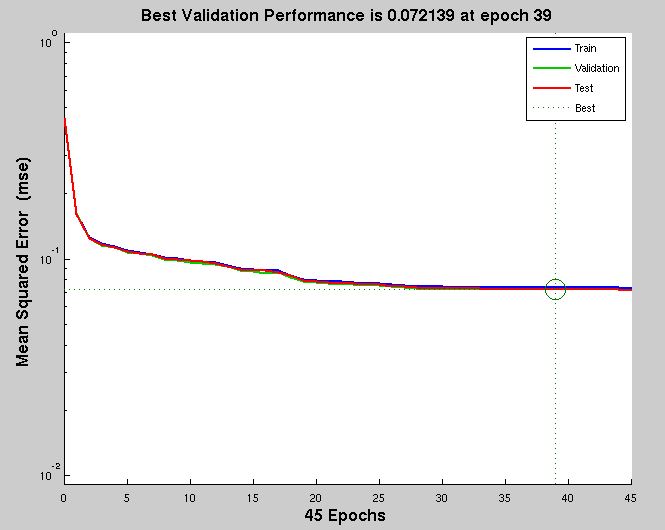
\includegraphics[width=15cm]{mse_3.png}
\end{center}
\vspace{0.5cm} 


On voit que le système à bien convergé. On a trouvé les meilleures poids possibles pour optimiser l'erreur minimum. Nous pouvons essayer maintenant avec les 10 fichiers restant.\pagebreak

\section{ANN test}

On passe en entrée les 5 colonnes (coefficients extrait) des 10 fichiers "wav" que l'on passe en entrée et on somme les sorties pour calculer les scores.  Voilà l'histogramme des scores :

\begin{center} 
\hspace{15cm}
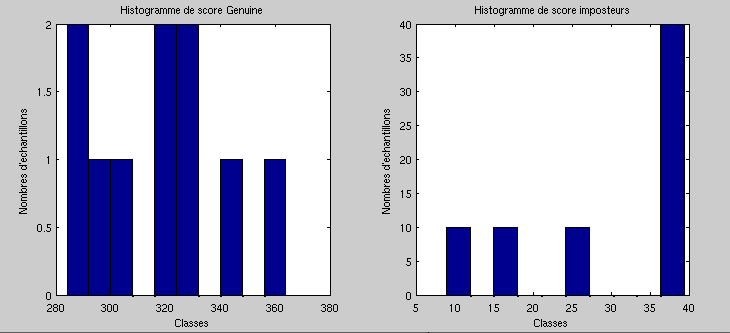
\includegraphics[width=15cm]{histo_3.png}
\end{center}
\vspace{0.5cm} 

On voit que les scores "genuine" sont entre 250-380 et les "impostors" sont entre 5-40. Voilà les graphiques de performances :

\begin{center} 
\hspace{15cm}
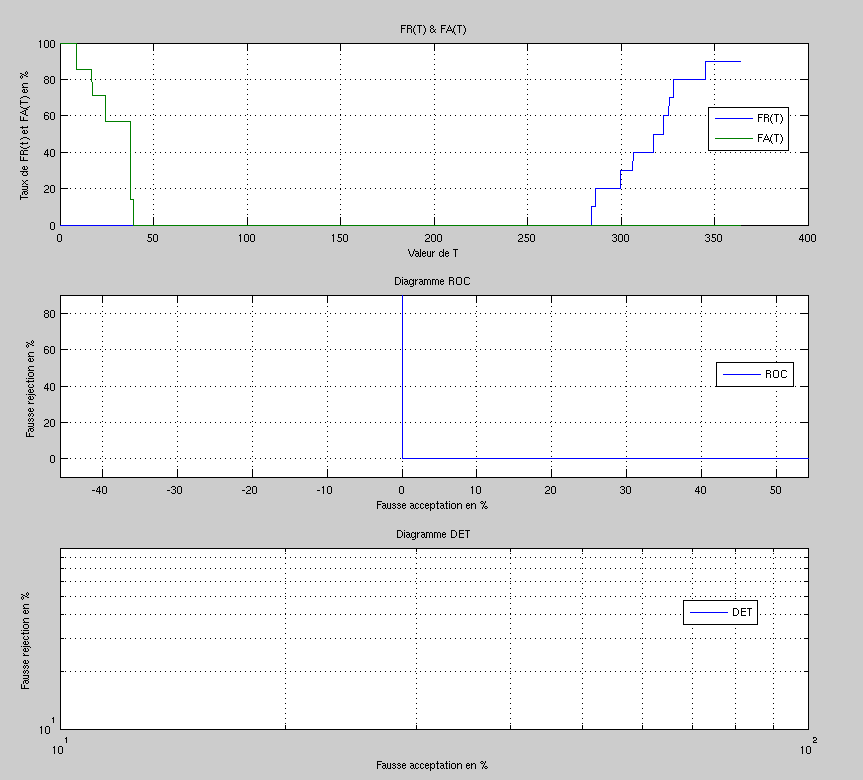
\includegraphics[width=13cm]{perf_3.png}
\end{center}
\vspace{0.5cm} 

\pagebreak
On remarque que les scores ne se recouvrent pas et que nous avons un système qui est parfait !




 


 


